\section{The Sommelier System}\label{design}

\myparagraph{Data Cleanup}

The data source I have used for my project is the wines database belonging to Decanter.com\cite{DecanterCom}. The database features professional ratings and tasting notes from as far back as 1986, and features wines from vintages as far back as 1917.

GRAPH: Distribution of vintages

The original database is highly inconsistent, displaying a mixture of design approaches and a variable quality of data. This is consistent with the fact that the database has been developed over a long period of time by a number of different developers with varying levels of skill, and that wine journalists making entries into the database have taken a number of idiosyncratic approaches to data entry.

Nevertheless there is a great deal of useful and interesting information in the database, as it contains ratings and/or tastings for over 33,000 wines.

The ``wine\_info'' table is a mixture of foreign keys joining to very small tables, such as ``wine\_info.type\_id'' joining to ``wine\_type.id'' where ``wine\_type'' is a table with only two attributes. This approach, stiving for a high degree of normalisation, contrasts with the fact that the same table also has the attribute ``second\_wine'', as string which only holds data in 450 of the 38762 entries in the table.

\myparagraph{Creating The Sommelier Dataset}

As well as containing a large amount of unreliable or incomplete data which was of little use to my project, the database's complex design would not lend itself to simple queries. 

Rather than using a large number of foreign key relations, which would necessitate a large number of joins at query time, I hoped to pare down the database to the minimum number of tables for the maximum ease of retrieval and manipulation. Figure \ref{fig:sommelierdb} shows the new database schema.

\begin{figure}[h!]
    \caption{Sommelier Database Schema}
    \centering
        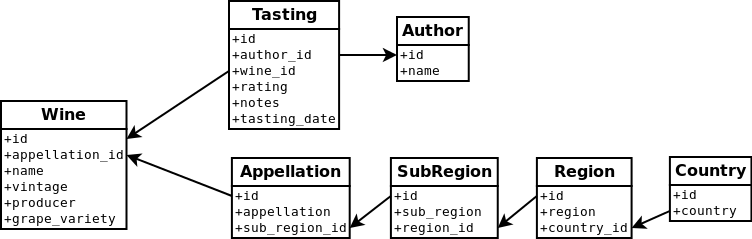
\includegraphics[width=14cm]{SommelierDB}
\end{figure}

Here I will describe that data and my reasoning for disregarding it...

The tables ``wine\_style\_narrow'' and ``wine\_style\_broad'' contained generic text descriptions for wine (``rich and creamy'', ``crisp and tangy'' etc.). I initially considered this to have potential for migration into tag data which I could reuse as part of my filtering. Unfortunately less than 6435 of the records in ``wine\_info'' had non-null values for their ``style\_narrow\_id'' field, and only 3397 had associations in the ``tasting'' table. 3397 was only around 10\% of the wines I expected to be working with in my migrated dataset, I reckoned this too low a proportion to be worthwhile.

The table ``wine\_style'' was rejected for the same reasons as those above.

The ``wine\_type'' table was ignored because no wines were related to it. Those wines with the ``type\_id'' field populated in the database were populated with keys which did not match any ``id'' in the type table.

The ``producers'' table was not disregarded, as there were over 20,000 wines with tasting notes and a producer record.

\myparagraph{The Author Problem}

The biggest shortcoming of the dataset is that the author of a tasting note is often not recorded. The number of wines with notes and known authors is only 1401, with there being 18 named authors on the system. 

Table \ref{table:authors} shows the distribution of tastings amongst authors, only 5 of which have tasted and rated more than 100 wines in the database.

\begin{table}[ht]
\caption{Authors of tasting notes and ratings}
\centering
\begin{tabular}{c c}
\\\hline\hline
Author               & Wines tasted, with notes and rating
\\\hline
Amy Wislocki         &            28 \\
Andrew Jefford       &           105 \\
Beverley Blanning MW &            13 \\
Carolyn Holmes       &             1 \\
Christelle Guibert   &           119 \\
Clive Coates MW      &             6 \\
David Peppercorn     &            44 \\
Gerald D Boyd        &             7 \\
Harriet Waugh        &           250 \\
James Lawther MW     &           226 \\
John Radford         &             2 \\
Josephine Butchart   &            24 \\
Norm Roby            &             4 \\
Rosemary George MW   &             6 \\
Serena Sutcliffe     &            31 \\
Stephen Brook        &            19 \\
Steven Spurrier      &           497 \\
\\\hline
\end{tabular}
\label{table:authors}
\end{table}

In some cases an author's initials or full name are recorded within the text of a tasting note. I decided that extracting and making use of these was impractical given the time constraints of this project.

DESCRIBE DATA SETS BEFORE AND AFTER

THE SOMMELIER DATASET

Having analysed the dataset and conceived an ideal schema, I needed to decide what the criteria to apply when extracting my new dataset from the source data.

Given that the purpose of the dataset is social recommendations, the first decision I made was to discard any wines without both tasting notes and a rating, whether.
